\documentclass{ximera}


\graphicspath{
  {./}
  {ximeraTutorial/}
  {basicPhilosophy/}
}

\newcommand{\mooculus}{\textsf{\textbf{MOOC}\textnormal{\textsf{ULUS}}}}

\usepackage{tkz-euclide}\usepackage{tikz}
\usepackage{tikz-cd}
\usetikzlibrary{arrows}
\tikzset{>=stealth,commutative diagrams/.cd,
  arrow style=tikz,diagrams={>=stealth}} %% cool arrow head
\tikzset{shorten <>/.style={ shorten >=#1, shorten <=#1 } } %% allows shorter vectors

\usetikzlibrary{backgrounds} %% for boxes around graphs
\usetikzlibrary{shapes,positioning}  %% Clouds and stars
\usetikzlibrary{matrix} %% for matrix
\usepgfplotslibrary{polar} %% for polar plots
\usepgfplotslibrary{fillbetween} %% to shade area between curves in TikZ
\usetkzobj{all}
\usepackage[makeroom]{cancel} %% for strike outs
%\usepackage{mathtools} %% for pretty underbrace % Breaks Ximera
%\usepackage{multicol}
\usepackage{pgffor} %% required for integral for loops



%% http://tex.stackexchange.com/questions/66490/drawing-a-tikz-arc-specifying-the-center
%% Draws beach ball
\tikzset{pics/carc/.style args={#1:#2:#3}{code={\draw[pic actions] (#1:#3) arc(#1:#2:#3);}}}



\usepackage{array}
\setlength{\extrarowheight}{+.1cm}
\newdimen\digitwidth
\settowidth\digitwidth{9}
\def\divrule#1#2{
\noalign{\moveright#1\digitwidth
\vbox{\hrule width#2\digitwidth}}}






\DeclareMathOperator{\arccot}{arccot}
\DeclareMathOperator{\arcsec}{arcsec}
\DeclareMathOperator{\arccsc}{arccsc}

















%%This is to help with formatting on future title pages.
\newenvironment{sectionOutcomes}{}{}


\title{Inaccurate}

\begin{document}

\begin{abstract}
suspicious
\end{abstract}
\maketitle



Graphs are wonderful tools!  They provide a global view and quickly highlight trends in behavior, maximum and minimum values, and sudden changes. \\

We rely on graphs quite a bit in our analysis. \\

Graphs are also inaccurate and untrustworthy. \\

They can't help it.  By their very construction, they hide important details and mislead us.





\begin{example}


Where do you think the horizontal asymptote is on this graph?

\begin{image}
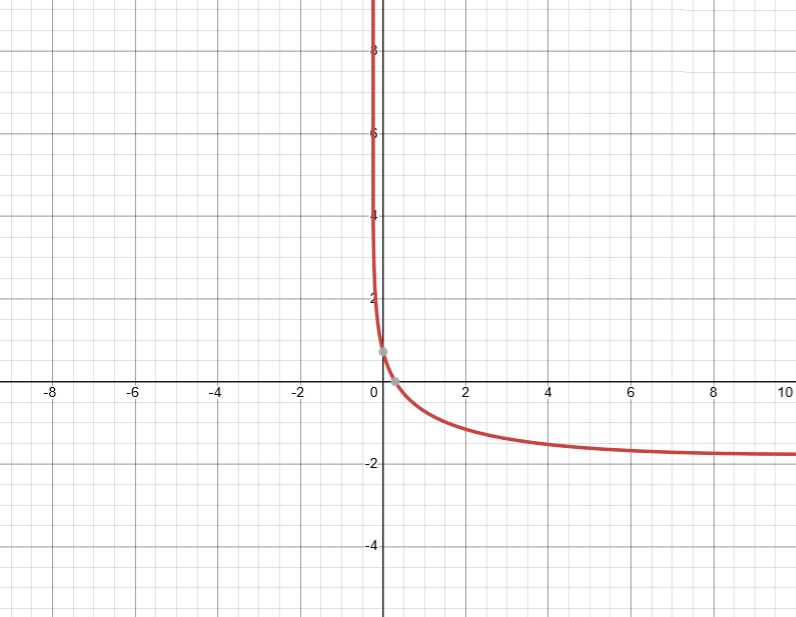
\includegraphics{pics/graph_1A.png}
\end{image}

It appears that the function levels off to an approximate value of $-1.75$. \\


Except, it doesn't.

\begin{image}
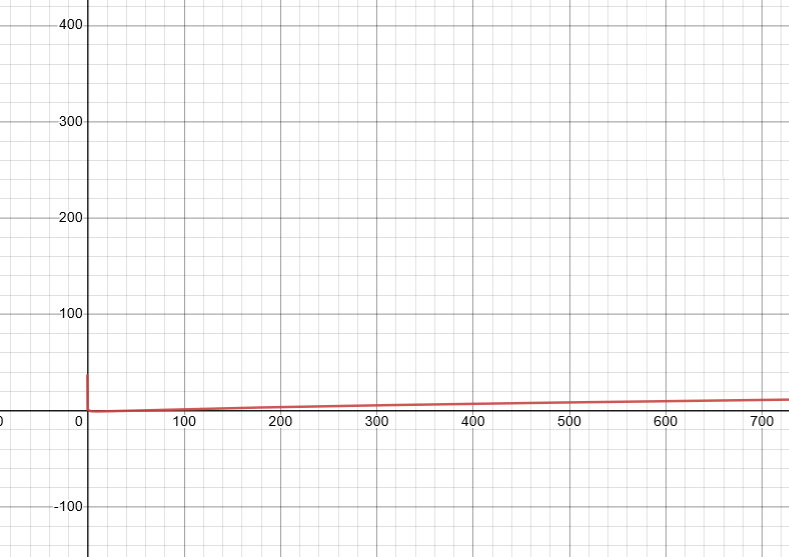
\includegraphics{pics/graph_1B.png}
\end{image}

This would have been immediately clear with algebra.

\[  \sqrt{\frac{x}{2}+2} - \ln(8x+2)      \]


\end{example}












\begin{example}


This graph has $x=2$ as a vertical asymptote.

\begin{image}
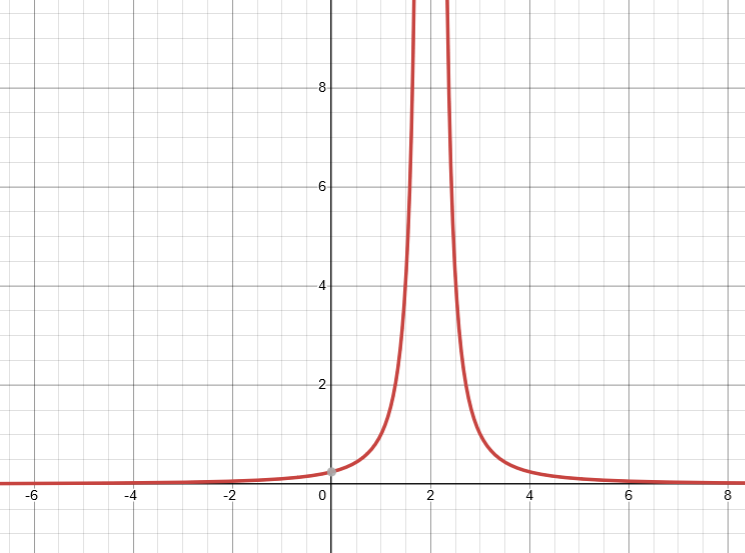
\includegraphics{pics/graph_2A.png}
\end{image}

It appears that $2$ is not in the domain. \\


Except, that is incorrect.

\begin{image}
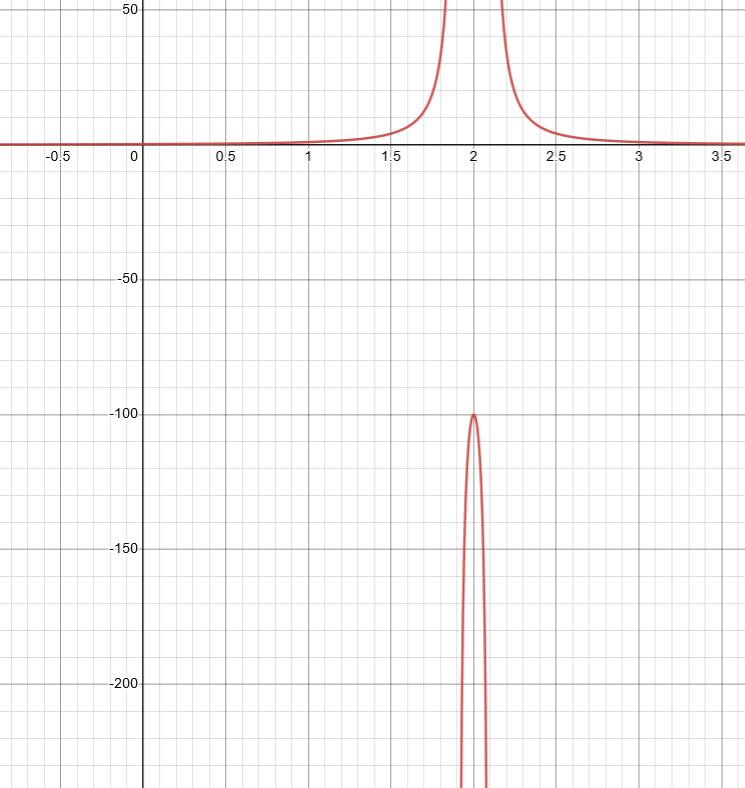
\includegraphics{pics/graph_2B.png}
\end{image}


$2$ is in the domain. $1.9$ and $2.1$ are not. \\


This would have been immediately clear with algebra.

\[  \frac{1}{(x-1.9)(x-2.1)}     \]


\end{example}


















\begin{example}


This function is decreasing on the interval $(-0.2, \infty)$.

\begin{image}
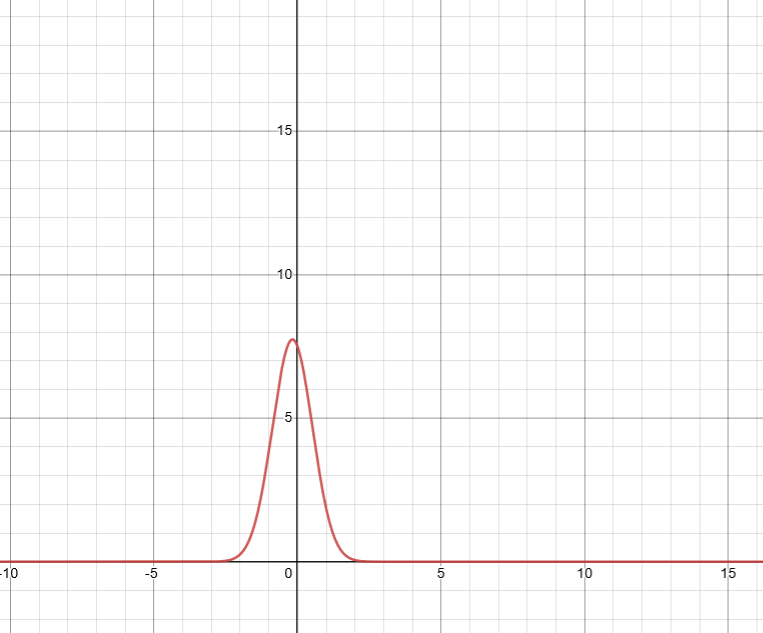
\includegraphics{pics/graph_3A.png}
\end{image}




Except, that is incorrect.

\begin{image}
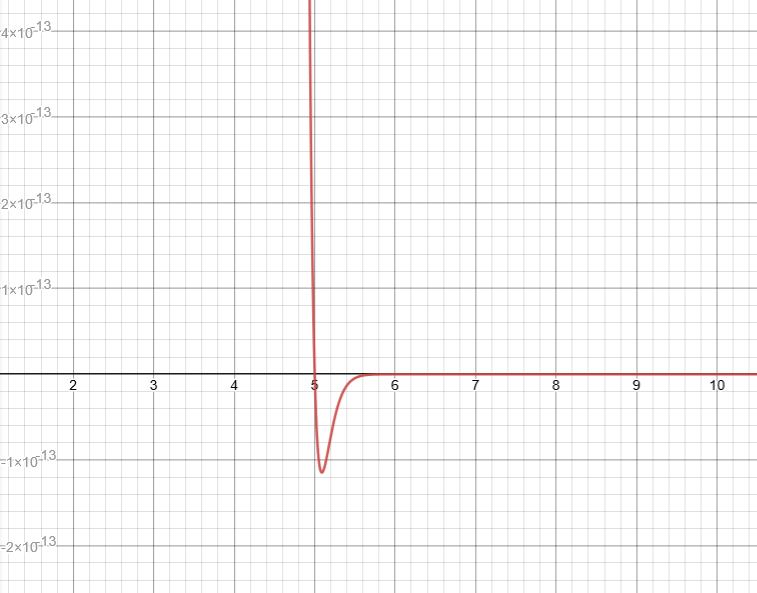
\includegraphics{pics/graph_3B.png}
\end{image}


This function actually has negative values and is actually increasing where it looked like it was decreasing. \\


Again, algebra would have hinted at this behavior.

\[  \frac{1}{4} e^{-x^2} (x-5)(x-6)     \]


\end{example}










\begin{example}


This function has different limiting values depending on which way you are looking.

\begin{image}
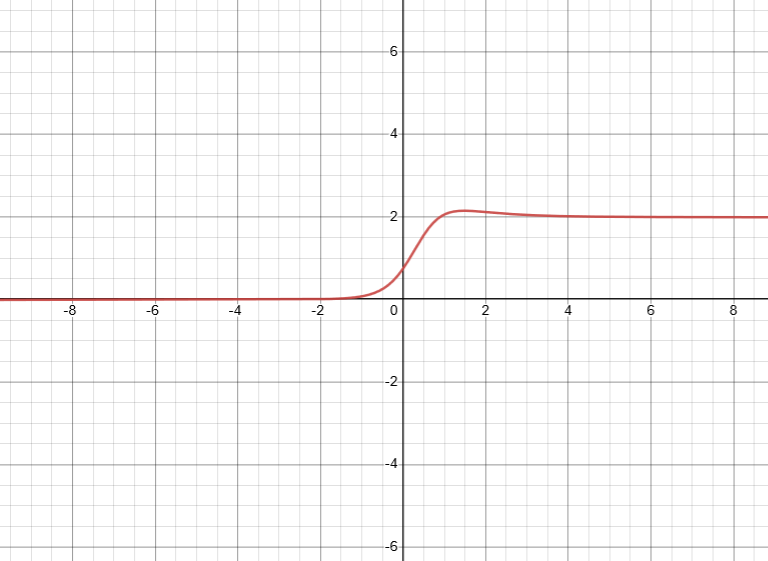
\includegraphics{pics/graph_4A.png}
\end{image}




Except, that this function is unbounded.

\begin{image}
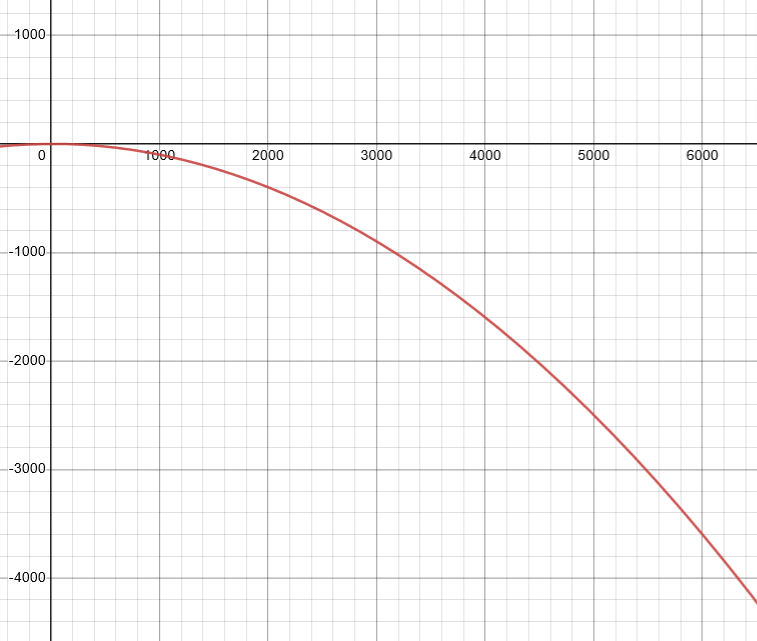
\includegraphics{pics/graph_4B.png}
\end{image}





Again, algebra would have hinted at this behavior.

\[  \frac{2+e^{-x}}{1+3 e^{-3x}} -\frac{x^2}{10000}     \]


\end{example}



Graphs are inherently inaccurate.  There is no way around that fact.  We love graphs and we use them all of the time. \\

We are also distrustful of graphs.  We are suspicous of graphs. \\

Graphs suggest, but we want algebraic verification. \\

Hence, algebra is our goal.












\begin{center}
\textbf{\textcolor{green!50!black}{ooooo=-=-=-=-=-=-=-=-=-=-=-=-=ooOoo=-=-=-=-=-=-=-=-=-=-=-=-=ooooo}} \\

more examples can be found by following this link\\ \link[More Examples of Graphical Analysis]{https://ximera.osu.edu/csccmathematics/precalculus1/precalculus1/graphicalAnalysis/examples/exampleList}

\end{center}





\end{document}
